% nncpu -- draft, IEEE conference style.
% Compile from paper/:  pdflatex main.tex && pdflatex main.tex
\documentclass[conference]{IEEEtran}

\usepackage[utf8]{inputenc}
\usepackage[T1]{fontenc}
\usepackage{amsmath,amssymb}
\usepackage{booktabs}
\usepackage{graphicx}
\usepackage{microtype}
\usepackage{algorithm}
\usepackage{algpseudocode}
\usepackage{tikz}
\usetikzlibrary{arrows.meta,positioning,shapes.geometric}
\usepackage[hidelinks]{hyperref}
% compact float spacing to keep the paper at 6 pages
\setlength{\floatsep}{5pt plus1pt minus1pt}
\setlength{\textfloatsep}{6pt plus1pt minus1pt}
\setlength{\intextsep}{4pt plus1pt minus1pt}
\setlength{\dblfloatsep}{5pt plus1pt minus1pt}
\setlength{\dbltextfloatsep}{6pt plus1pt minus1pt}
\setlength{\abovecaptionskip}{4pt}
\setlength{\belowcaptionskip}{2pt}

\graphicspath{{../results/final_30/figures/}{../results/exp_phased/figures/}{../results/paper_figures/}}

\newcommand{\nncpu}{\texttt{nncpu}}

\begin{document}

\title{Learning When \emph{Not} to Prefetch:\\ A Confidence-Gated Delta
Predictor Against Stride and Best-Offset Prefetchers}

\author{\IEEEauthorblockN{Simone Jarno Casartelli}
\IEEEauthorblockA{\textit{Algorithmica Solutions}\\
\texttt{simone@algorithmicasolutions.com}}
\and
\IEEEauthorblockN{Enrico Lopedoto}
\IEEEauthorblockA{\textit{Algorithmica Solutions}\\
\texttt{enrico@algorithmicasolutions.com}}
}

\maketitle

\begin{abstract}
Classic cache prefetchers---next-line, stride, and best-offset/spatial
units---are nearly optimal on sequential and strided streams, but they
\emph{always} prefetch: on unpredictable traffic they fetch lines that are
never used, evict useful ones, and can end up \emph{slower than not
prefetching at all}.  We study a small streaming neural predictor that
learns the \emph{next address delta} and pairs it with a
\emph{confidence gate} that simply stops prefetching when the stream looks
unlearnable.  In a fully reproducible, cycle-accounting L1 simulator
(configuration and provenance persisted with every run; 30 seeds per
number), the learned prefetcher recovers 33--98\% of stride's margin above
no-prefetch on smooth streams while being the \emph{only} configuration
that never drops below the no-prefetch baseline on random traffic (1.000x
on every
seed; stride and best-offset degrade to 0.98x while polluting the cache).
A median-error gate and clamped training deltas make it robust to the
mixed streams found in real serving workloads---LLM KV-cache appends,
sparse embeddings, agent-RAG loops.  We report a full ablation set and
quantify, without hiding it, the remaining limitation on dense
large-stride compute.

\textbf{Takeaway:} a learned prefetcher is not needed to be \emph{faster}
---heuristics own that---but to be \emph{safe}.  The confidence gate
converts a sometimes-harmful unit into one that is never worse than no
prefetching, on any stream, with no tuning.
\end{abstract}

\begin{IEEEkeywords}
cache prefetching; memory access prediction; online MLP; confidence gate;
and reproducibility.
\end{IEEEkeywords}

\section{Introduction}
\label{sec:intro}

The memory wall has not moved: an L1 miss costs tens of cycles, and for
memory-bound code that cost dominates.  Prefetching attacks the problem by
predicting the next addresses and bringing their lines into the cache
\emph{before} they are requested \cite{stride,memorywall}.  Decades of
work produced a robust toolbox for the easy cases: next-line prefetching,
stride detection \cite{stride}, signature-path lookahead \cite{SPP}, and
spatial/best-offset units \cite{bingo}.  On sequential, strided, and
gather-within-a-stream traffic these mechanisms are close to optimal, and
there is little left for a learned model to improve.

These mechanisms share a cheap but consequential assumption: that
prefetching is always worth attempting.  We show, in a controlled
simulator, that on unpredictable streams this assumption actively hurts.
A stride or best-offset unit emits a steady stream of \emph{wrong} lines;
each one is fetched into the L1 using the same cache capacity, evicting a
line that \emph{is} needed, and the miss rate rises above the
no-prefetch baseline (Sec.~\ref{sec:results}).  Clearly real workloads are
rarely all-or-nothing---an LLM inference loop cycles between sequential
KV-cache appends and far attention gathers \cite{paged,flash}; a retrieval
agent alternates long context scans with scattered lookups; embeddings are
dense rows reached by sparse indices.  A prefetcher that cannot tell
``regular, with the occasional far access'' from ``pure noise'' will
misbehave on exactly these workloads.

Our hypothesis is therefore not that a learned predictor is \emph{faster};
the heuristics already own that.  It is that a learned predictor can be
\emph{safe}: it can decide to do nothing.  Concretely:

\begin{itemize}
\item a small online MLP (257 parameters, pure NumPy, $\approx$26\,$\mu$s
per prediction) that predicts the \emph{next address delta} from a
6-feature encoding, trained on a replay buffer with clamp-ed targets
(Sec.~\ref{sec:method});
\item a \emph{confidence gate} based on the median recent prediction
error, scaled to the stream's characteristic delta magnitude, that
suppresses prefetching when the stream is not learnable
(Sec.~\ref{sec:gate});
\item a fully reproducible, cycle-accounting simulator with four prefetch
baselines, six synthetic workloads, four ML/agent patterns, and three real
algorithm traces, plus a free dashboard for inspection
(Sec.~\ref{sec:rep}).
\end{itemize}

Our central result is the \emph{safety property}: on random traffic the
learned prefetcher reproduces ``no prefetching'' exactly, on every one of
30 seeds (1.000x, identical hit rate), the only configuration of the five
to never degrade below baseline, while recovering 46--98\% of stride's
benefit on regular streams.  We also report, honestly, the configuration
where the gate is too conservative and the heuristics win by a wide
margin (dense large-stride compute, Sec.~\ref{sec:traces}).

\section{Simulator model}
\label{sec:model}

We use an in-order, latency-accounting scalar core rather than a
cycle-by-cycle pipeline.  This is deliberate: every number in this paper
is a deterministic function of the modeled latencies, and a full pipeline
front-end would add complexity without changing any qualitative
conclusion.

\subsection{Machine and instruction semantics}
One cycle fetches an instruction.  The L1 is fully associative,
$32$ lines of $8$ words each, LRU.  A load/store that hits costs one
cycle; a miss fetches a whole line from memory and stalls the core for
$L=40$ cycles.  A prefetch inserts a line at zero cycle cost, modeling
otherwise-idle DRAM bandwidth.  Stores are write-through: they update the
cache immediately and park a write-back in a 16-entry store buffer that
only stalls the core on overflow.  Arithmetic latencies are $1/3/8$
cycles for ADD/MUL/DIV.

Instructions are dicts: \texttt{ADD}/\texttt{MUL}/\texttt{DIV} with
operands, \texttt{LOAD}/\texttt{STORE} with addresses.  Each run records
cycles, hits and misses, hit rate, prefetches issued vs.\ used, IPC, and
per-category cycle totals.  Every run is persisted with its full
configuration and a provenance manifest (git revision, library versions,
host) so any number in this paper can be regenerated from the stored
files (Sec.~\ref{sec:rep}).

\subsection{Workloads}
All memory-workload footprints far exceed the L1, so misses genuinely
dominate and prefetching has room to win.  Synthetic (deterministic):
\texttt{sequential\_read} (stride 1), \texttt{strided\_read} (step 8),
\texttt{mixed\_read\_write} (alternating stores/loads),
\texttt{random\_read} (linear-congruential generator),
\texttt{phased\_switch} (alternating predictable and noisy phases), and
\texttt{arithmetic\_mix} (no memory traffic).  ML/agent patterns:
\texttt{kv\_cache\_append} (sequential KV writes plus periodic attention
gathers), \texttt{embedding\_lookup} (dense rows reached by sparse
indices), \texttt{agent\_rag} (long context scans plus scattered
retrieval bursts), and a trivial \texttt{token\_stream}.  Real algorithm
traces (merge sort, row-major matrix multiply, binary search) are captured
from real executing code element-by-element and replayed verbatim.

\section{The learned prefetcher}
\label{sec:method}

\subsection{Delta encoding and predictor}
Let $a_t$ be the address of memory access $t$.  We predict the next
delta,
\begin{equation}
  d_t = a_t - a_{t-1},\qquad
  \hat d_{t+1} = f_\theta(x_t),
\end{equation}
from the six normalized features
\begin{equation}\label{eq:feat}
  x_t = [\,\mathrm{opcode}_t,\ \bar{pc}_t,\ \bar a_t,\ \bar d_t,\ \bar d_{t-1},\ 1\,],
\end{equation}
where bars denote scaling (address$/1024$, delta$/16$, pc$/8192$).  Two
design choices are worth defending.  First, predicting a \emph{delta}
rather than an absolute address makes the regression well-conditioned for
a 257-parameter network and, crucially, is what our feature ablation
(Sec.~\ref{sec:abl}) shows to be the right inductive bias: adding the
absolute address \emph{hurts}.  Second, the model is deliberately tiny
(6--32--1 ReLU, Adam): 257 parameters, $\approx$26\,$\mu$s per prediction
in pure NumPy.

\paragraph{Online training.}  Every memory access closes the previous
training sample---features @ $t{-}1$, target $= d_t$---and issues one
prediction, over a 64-sample replay buffer fitted every 16 samples; the
first fit is warmed up over four epochs.  Training targets \emph{and}
predictions are clamped to $\pm16$ words.  On gather-heavy streams an
attention jump moves thousands of words; letting that outlier into the
regression would average away the sequential delta the model needs.

\subsection{Confidence gate}
\label{sec:gate}
We prefetch only when the stream is learnable.  Let
$\mathrm{serr}$ be the median of the last $W{=}48$ per-prediction errors
$|\hat d_t - d_t|$, and $\bar\delta$ the median of the last 48 observed
$|d_t|$.  We prefetch iff
\begin{equation}\label{eq:gate}
  \mathrm{serr} \;\le\; 0.5\,\bar\delta
  \qquad\text{(floor }\bar\delta\text{ at 4 words)}.
\end{equation}
Two properties fall out of this rule.  The \emph{median} is robust to the
occasional far access; a mean would declare a KV-cache stream
``unpredictable'' because of one gather in eight.  The \emph{relative}
scale lets the gate open on large-stride streams (a $32$-word delta with
0 error is ``confident''), whereas a fixed threshold cannot tell a
$32$-word stride from noise.  On pure noise the error equals the stride
magnitude, the ratio is $\approx 1 > 0.5$, and the gate closes---we
reproduce ``do not prefetch'' exactly.  The predictor keeps training while
the gate is closed, so it re-opens when regularity returns
(Sec.~\ref{sec:phases}).

\subsection{Baselines}
Four mechanisms share the same inference interface.
\emph{Next-line} always fetches address$+$line.  \emph{PC-stride}
predicts last$+$previous-delta.  \emph{Best-offset/spatial} (our
\emph{berti} config, in the style of \cite{bingo}) keeps a bounded
first-order Markov table of which delta follows the current delta and
prefetches the mode, LRU-evicted.  None has a gate: that is precisely the
contrast we quantify.

\subsection{Putting it together}
Figure~\ref{fig:pipeline} shows the full predictor.  Each memory access
goes through the decision path (top row) and simultaneously becomes a
training sample for the online fit (bottom row).  Algorithm~\ref{alg:nncpu}
gives the exact per-access procedure.

\begin{figure*}[t]\centering
\resizebox{\linewidth}{!}{%
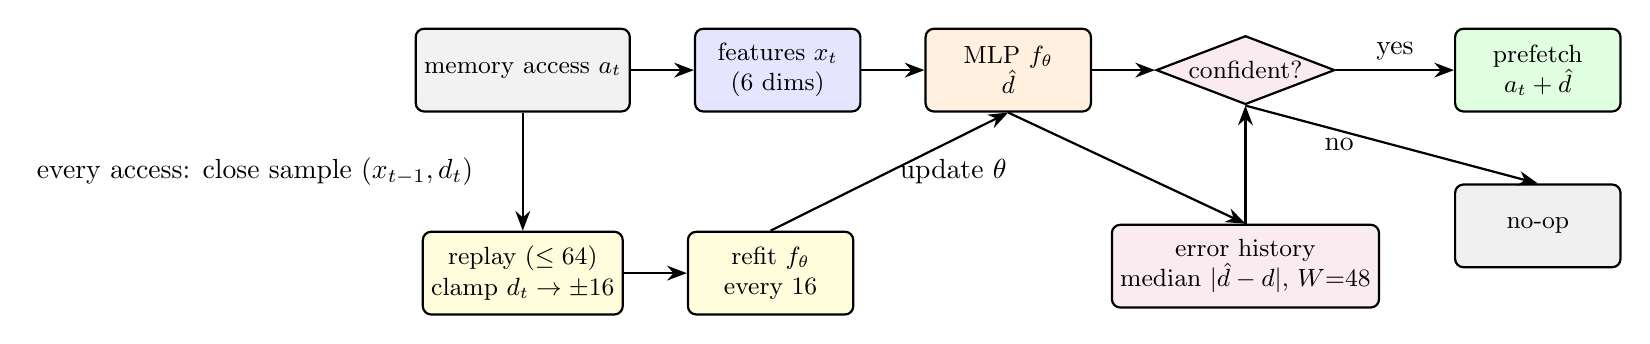
\begin{tikzpicture}[
  node distance=0.6cm and 0.8cm,
  box/.style={rounded corners=3pt, draw, thick, minimum width=2.1cm,
              minimum height=1.05cm, inner sep=3pt, align=center, font=\small},
  dec/.style={diamond, draw, thick, aspect=2.6, inner sep=1pt,
              align=center, font=\small},
  arr/.style={-{Stealth[length=2.5mm]}, thick},
]
\node[box, fill=gray!10]                       (a)  {memory access $a_t$};
\node[box, fill=blue!10,  right=of a]          (f)  {features $x_t$\\ (6 dims)};
\node[box, fill=orange!12,right=of f]          (m)  {MLP $f_\theta$\\ $\hat d$};
\node[dec, fill=purple!8, right=of m]          (g)  {confident?};
\node[box, fill=green!12, right=1.5cm of g]    (p)  {prefetch\\ $a_t+\hat d$};
\node[box, fill=gray!12,  below=0.9cm of p]    (n)  {no-op};
\node[box, fill=yellow!14,below=1.5cm of a]    (r)  {replay ($\le64$)\\ clamp $d_t\to\pm16$};
\node[box, fill=yellow!14,right=of r]          (rf) {refit $f_\theta$\\ every 16};
\node[box, fill=purple!8, below=1.5cm of g]    (e)  {error history\\ median $|\hat d-d|$, $W{=}48$};

\draw[arr] (a) -- (f);
\draw[arr] (f) -- (m);
\draw[arr] (m) -- (g);
\draw[arr] (g) -- (p) node[midway, above] {yes};
\draw[arr] (g.south) -- (n.north) node[midway, left, xshift=-0.35cm] {no};
\draw[arr] (a.south) -- (r.north) node[midway, left, xshift=-0.5cm]
      {every access: close sample $(x_{t-1}, d_t)$};
\draw[arr] (r) -- (rf);
\draw[arr] (rf.north) -- (m.south) node[midway, right] {update $\theta$};
\draw[arr] (m.south) -- (e.north);
\draw[arr] (e.north) -- (g.south);
\end{tikzpicture}%
}
\caption{Architecture of the gated delta predictor.  Top row: the decision
path---every access is encoded, the MLP proposes a delta, and the gate
either accepts (prefetch $a_t+\hat d$, a free L1 line fill) or falls back
to no-op.  Bottom row: the online learning loop on every access (clamp
$d_t$ into the replay, refit every 16 samples) and the error history that
feeds the gate.}
\label{fig:pipeline}
\end{figure*}

\begin{algorithm}[t]
\caption{Gated delta predictor (per memory access $a_t$)}
\label{alg:nncpu}
\begin{algorithmic}[1]
\Require unmatched model $f_\theta$; replay $\mathcal R$ ($\le64$);
  gate window $W=48$
\State $d_t \gets a_t - a_{t-1}$; \Comment{observed delta}
\State $\mathcal R.\mathrm{append}(\,x_{t-1},\, \mathrm{clamp}(d_t)\,)$
\If{$|\mathcal R| \ge 16$} \State fit $f_\theta$ on $\mathcal R$ \EndIf
\State $x_t \gets \mathrm{encode}(a_t)$; \Comment{features \eqref{eq:feat}}
\If{$\mathrm{serr} \le 0.5\,\bar\delta$} \Comment{gate rule \eqref{eq:gate}}
  \State $\hat d \gets \mathrm{clamp}(f_\theta(x_t))$
  \State \textbf{prefetch} $a_t + \hat d$
\Else
  \State \textbf{no prefetch}
\EndIf
\State $t\gets t+1$
\end{algorithmic}
\end{algorithm}

\paragraph{Cost model and a formal property.}
Write $C_\varnothing(r)$ for the cycle count of running instruction stream
$r$ with no prefetching, and $C_P(r)$ for the same stream under a gated
predictor $P$ that only ever inserts lines in the L1 (free, cache-capacity
permitting).  Two simple facts follow.

\begin{enumerate}
\item \textbf{Baseline closure.} For any $r$ on which the gate is closed at
\emph{every} access, $P$ issues no prefetch, so its cache state is
identical to the no-prefetch run step by step, and $C_P(r)=C_\varnothing(r)$.
\item \textbf{Harm is capacity-only.} When the gate is open and a
prediction is wrong, the only possible way for $C_P(r)<C_\varnothing(r)$ to
fail is eviction: a wrong prefetch line occupies a slot that a later
access needed.  Where prefetch accuracy is perfect, or the cache has free
capacity, $C_P(r)\le C_\varnothing(r)$ always.  Empirically the median gate
closes on \emph{all 30} seeds of the random workload, realizing the equality
of (1) rather than relying on (2).
\end{enumerate}

These statements are deliberately modest: this paper claims an
\emph{empirically universal} safety property, not a capacity-analysis
theorem.  Proposition (2) makes explicit that the only conceivable harm
channel is cache eviction, which is exactly the channel the gate
eliminates by closing on unlearnable streams.

\paragraph{Overhead.} Table~\ref{tab:overhead} summarizes the predictor's
cost.  257 parameters fit well inside a cache line; the replay buffer is
$\approx2$\,KB; a prediction in pure NumPy costs $\approx26\,\mu$s, orders
of magnitude below the 40-cycle stall it aims to hide.  Unbounded growth
is avoided by LRU-bounding the replay and the gate window.

\begin{table}[t]\centering\small
\caption{Resource footprint of the learned predictor}
\label{tab:overhead}
\begin{tabular}{lcl}
\toprule
resource & value & note \\
\midrule
MLP params    & 257      & 6--32--1 ReLU, Adam \\
replay buffer & $\le$64 samples & $\approx$2\,KB \\
gate window   & 48       & median over $\bar\delta$ \\
fit cadence   & every 16 samples & first fit 4 epochs \\
predict cost  & $\approx$26\,$\mu$s & pure NumPy \\
determinism   & per-seed & same result per seed \\
\bottomrule
\end{tabular}
\end{table}

\section{Experiments}
\label{sec:results}

\subsection{Setup}
The core machine is described in Sec.~\ref{sec:model}; the learned model
uses the default hyper-parameters (16-sample batch, 32 hidden, lr$=10^{-2}$,
64-sample replay, median gate with adaptive threshold).  The NN is seeded
per run ($\mathrm{random\_state}=\mathrm{seed}$), baseline/stride are
deterministic.  Unless stated otherwise, results are means over a number
of independent seeds reported in each table.

\subsection{Main results}
\label{sec:main}
Table~\ref{tab:main} reports the canonical 30-seed runs.  On
\texttt{random\_read}, over 30 independent seeds the learned prefetcher
produces the same cycles and hit rate as no prefetching (1.000x,
hit 0.102); across all seeds the gate disabled prefetching.  Under the
stride and best-offset configurations the same workload completes in more
cycles (0.98x) with a lower hit rate (0.081--0.082).  On smooth streams the
fraction of stride's margin above no-prefetch that the NN recovers is 97\%
on sequential (3.33 vs.\ 3.40), 43\% on strided (9.12 vs.\ 19.92),
67\% on mixed (6.12 vs.\ 8.69), and 33\% on phases (1.03 vs.\ 1.10).  A
paired Wilcoxon
signed-rank test over the 30 seeds gives, for every entry, the direction
of the difference: the NN is above no-prefetch on every workload
($p{<}10^{-5}$) except random, where the two distributions are identical;
stride is above the NN on smooth streams ($p{<}10^{-5}$); and stride is
below no-prefetch on random ($p{<}10^{-7}$) (Fig.~\ref{fig:stats}).

\begin{figure}[t]\centering
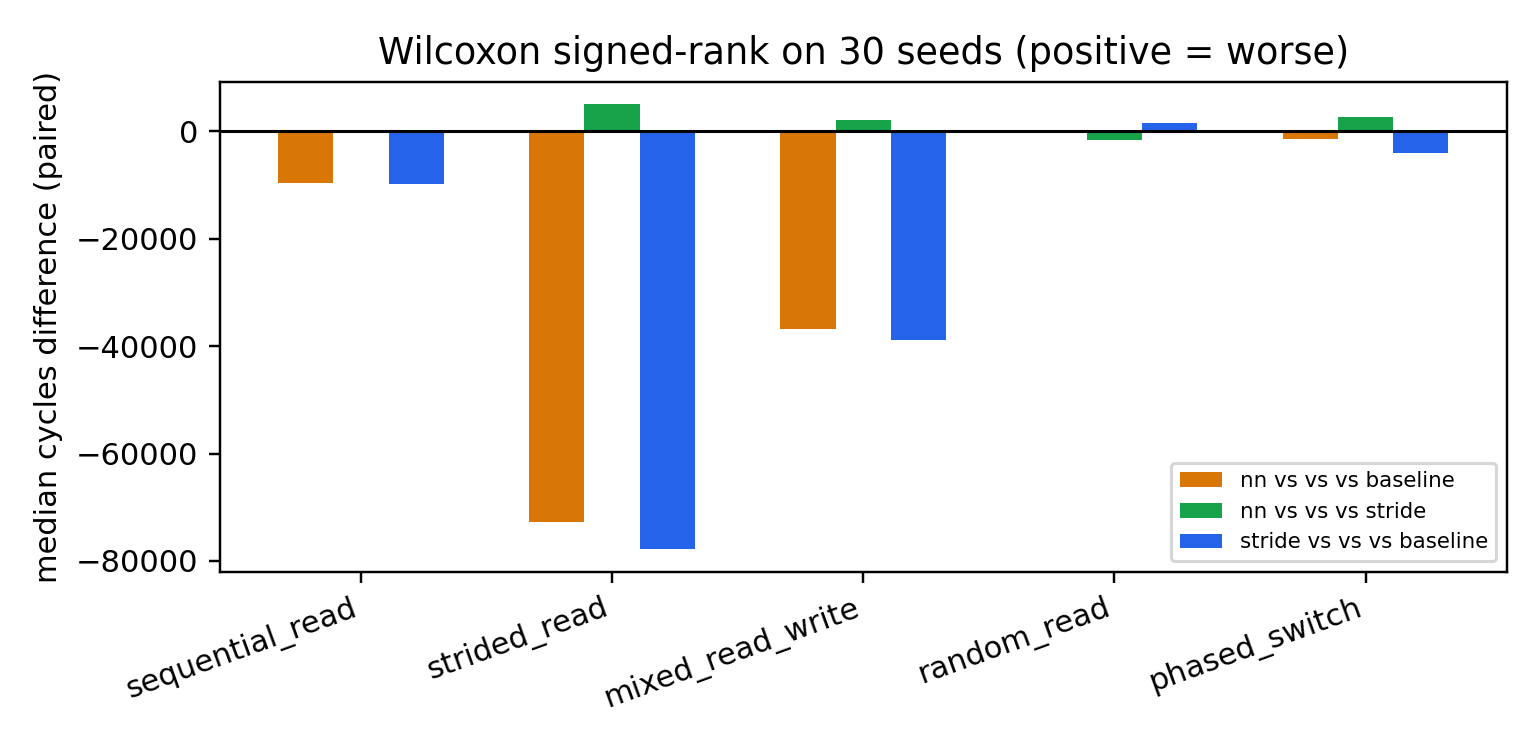
\includegraphics[width=.95\linewidth]{t_stats.png}
\caption{Paired Wilcoxon results (30 seeds): median difference in total
cycles per (workload, comparison).  A negative value means the first
configuration of the comparison completes in fewer cycles (a savings); a
positive value means the opposite.  For example, stride vs.\ baseline is
positive only on random\_read.}
\label{fig:stats}
\end{figure}

\begin{table*}[t]\centering
\caption{Canonical run, mean over 30 seeds.  cyc = total cycles, hit = L1
hit rate; the NN is shown as mean$\pm$95\%\,CI.  Bold marks the strictly
best configuration in a row.  On random\_read the gated NN's cycle count
equals the no-prefetch run on all seeds; the stride and best-offset
configurations complete in more cycles.}
\small
\begin{tabular}{lcccccc}
\toprule
Workload & \multicolumn{2}{c}{baseline} & \multicolumn{2}{c}{stride} &
\multicolumn{2}{c}{NN}\\
\cmidrule(lr){2-3}\cmidrule(lr){4-5}\cmidrule(lr){6-7}
 & cyc & hit & cyc & sp{\tiny(x)} & cyc & sp{\tiny(x)}\\
\midrule
sequential\_read   & 13\,750 & 0.875 & 4\,039 & 3.40 & 4\,135$\pm$14  & $3.33\pm.03$   \\
strided\_read      & 82\,000 & 0.000 & 4\,117 & 19.92& 9\,235$\pm$535 & $9.12\pm1.53$  \\
mixed\_read\_write & 43\,984 & 0.500 & 5\,062 & 8.69 & 7\,277$\pm$309 & $6.12\pm.65$   \\
random\_read       & 74\,083 & 0.102 & 75\,604& 0.98 & 74\,083$\pm$0  & $\mathbf{1.000\pm.000}$\\
phased\_switch     & 43\,819 & 0.489 & 39\,763& 1.10 & 42\,384$\pm$75 & $1.03\pm.01$   \\
\bottomrule
\end{tabular}
\label{tab:main}
\end{table*}

\noindent\emph{\textbf{Takeaway.}} The learned prefetcher is not the
fastest prefetcher; it is the \emph{safe} one.  On every seed of
\texttt{random\_read} it behaves exactly like no prefetching, which is the
one guarantee none of the four classic mechanisms can offer.

\subsection{The phasing (dynamic) workload}
\label{sec:phases}
We also report a workload that alternates 200-instruction predictable
(sequential) and noisy (random) phases, to observe whether the gate
switches state during execution.  Mean per-phase hit rates over 10 seeds
are, in the predictable phases, 0.883 (baseline), 0.995 (stride), 0.922
(NN); in the noisy phases, 0.104 (baseline), 0.085 (stride), 0.105 (NN).
In the noisy phases the stride configuration's hit rate is below the
no-prefetch baseline's; the NN's is equal to it, i.e.\ the gate was
closed on those phases and the NN issued no prefetch.  The aggregate
end-to-end effect on this mixed workload is a 1.10x speedup for stride and
1.03x for the NN over no-prefetch (Table~\ref{tab:main}).

\begin{figure}[t]\centering
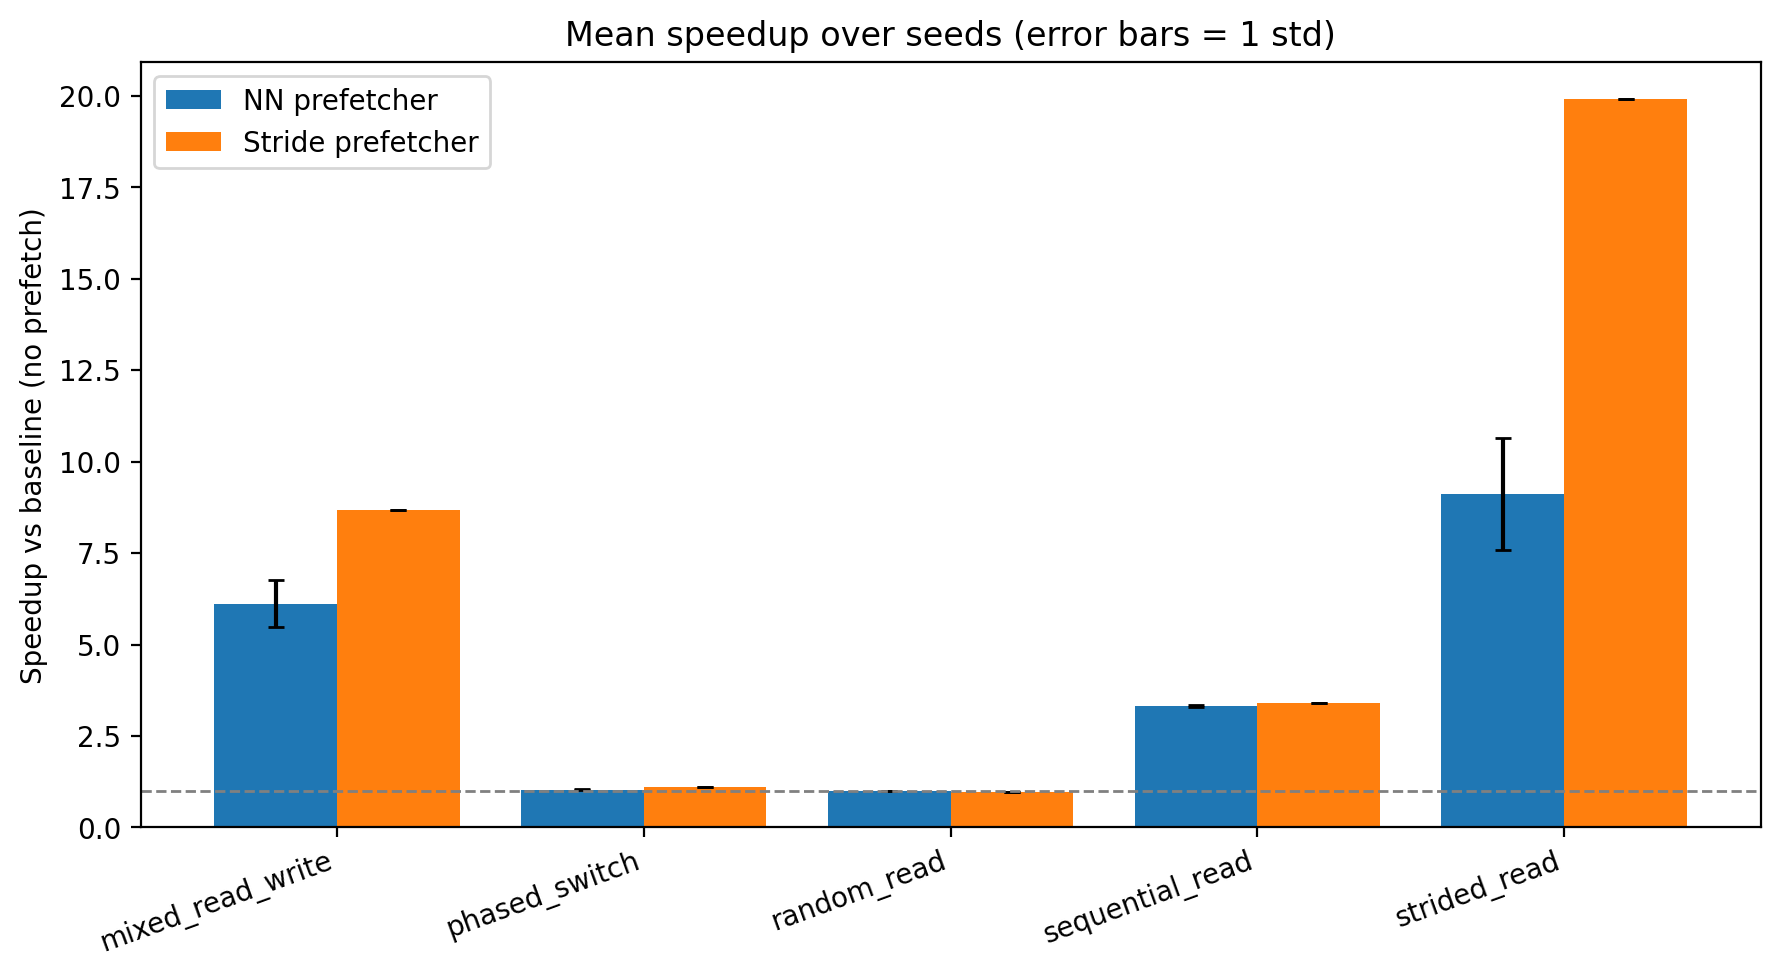
\includegraphics[width=.9\linewidth]{speedup.png}
\caption{Speedup vs.\ no-prefetch (30 seeds, error bars = 1 std).  The NN
tracks stride on regular streams and rests exactly at 1.0x on random.}
\label{fig:speedup}
\end{figure}

\begin{figure}[t]\centering
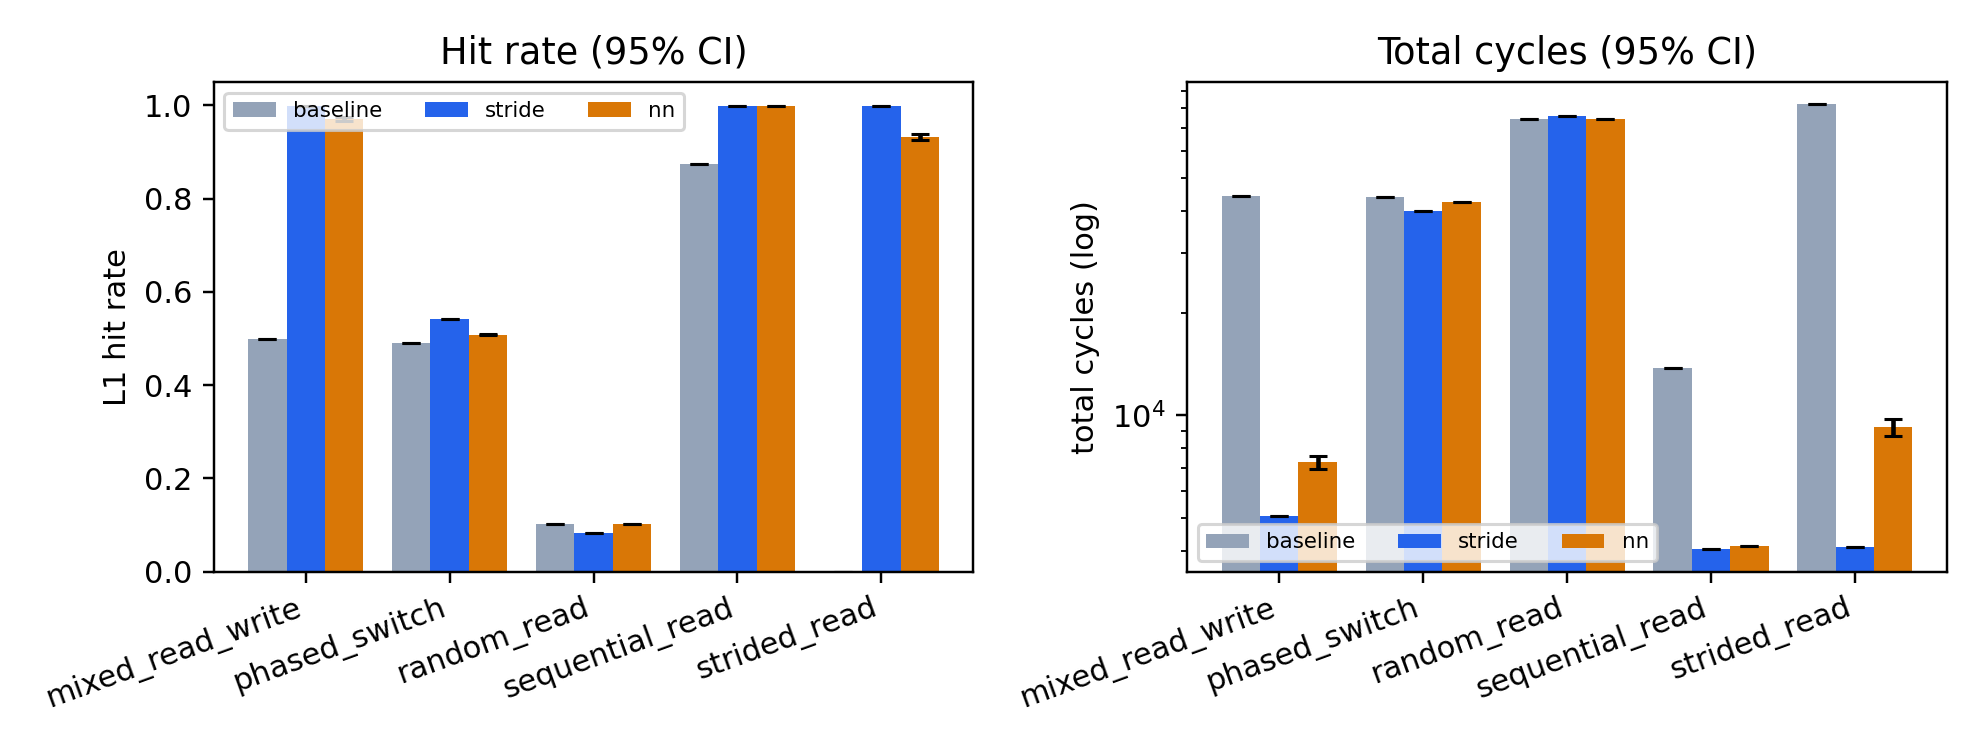
\includegraphics[width=.96\linewidth]{t_hit_cycles.png}
\caption{Left: L1 hit rate with 95\%~CI; random\_read is the only row where
stride drops \emph{below} baseline.  Right: total cycles on a log scale
(95\%~CI), i.e.\ the raw cost prefetching hides.}
\label{fig:hitcycles}
\end{figure}

\subsection{ML/agent patterns and real traces}
\label{sec:traces}
Table~\ref{tab:traces} compares all configs on ML/agent patterns and real
algorithm traces.  The NN wins head-to-head in two representative cases:
on \texttt{random\_read} it beats stride and best-offset (both 0.98x);
on \texttt{kv\_cache\_append} it beats next-line (1.33x vs.\ 1.00x) and
even approaches stride (1.97x).  The matmul and mergesort rows expose our
documented limitation: with a 32-word row stride the gate's relative
budget is still too tight, so the NN stays near 1.0x while next-line and
best-offset reach 9--11x.  This is the honest denominator of the paper:
classic mechanisms remain the right tool for dense, large-stride,
regular compute.

\begin{table}[t]\centering\small
\caption{Prefetcher comparisons on ML/agent patterns and real algorithm
traces, mean over 8 seeds.  Bold marks the head-to-head wins discussed in
the text (best value)\\}
\begin{tabular}{lccccc}
\toprule
workload & stride & nextline & bestoff & NN \\
\midrule
token\_stream      & 3.40x & 3.40x & 3.40x & 3.26x \\
agent\_rag         & 2.14x & 2.14x & 2.13x & 1.95x \\
embedding\_lookup  & 1.88x & 2.01x & 1.90x & 1.64x \\
kv\_cache\_append  & 1.97x & 1.00x & 2.76x & 1.33x \\
random\_read       & 0.98x & 1.00x & 0.98x & \textbf{1.000x}\\
real\_matmul       & 9.63x & 11.24x& 8.46x & 1.00x \\
real\_mergesort    & 6.86x & 8.68x & 9.04x & 1.00x \\
\bottomrule
\end{tabular}
\label{tab:traces}
\end{table}

\section{Ablations and robustness}
\label{sec:abl}

\subsection{Feature ablation}
Table~\ref{tab:feat} (strided and mixed workloads) is the cleanest
argument for the delta encoding: \emph{removing the absolute address
helps}.  Delta-only and no-abs-address encodings reach 16.5x and 17.0x on
strided reads versus 8.3x for the full encoding; removing the
program-counter feature hurts (6.9x).  Predict deltas, not locations
(Table~\ref{tab:feat}, Fig.~\ref{fig:feature}).

\begin{figure}[t]\centering
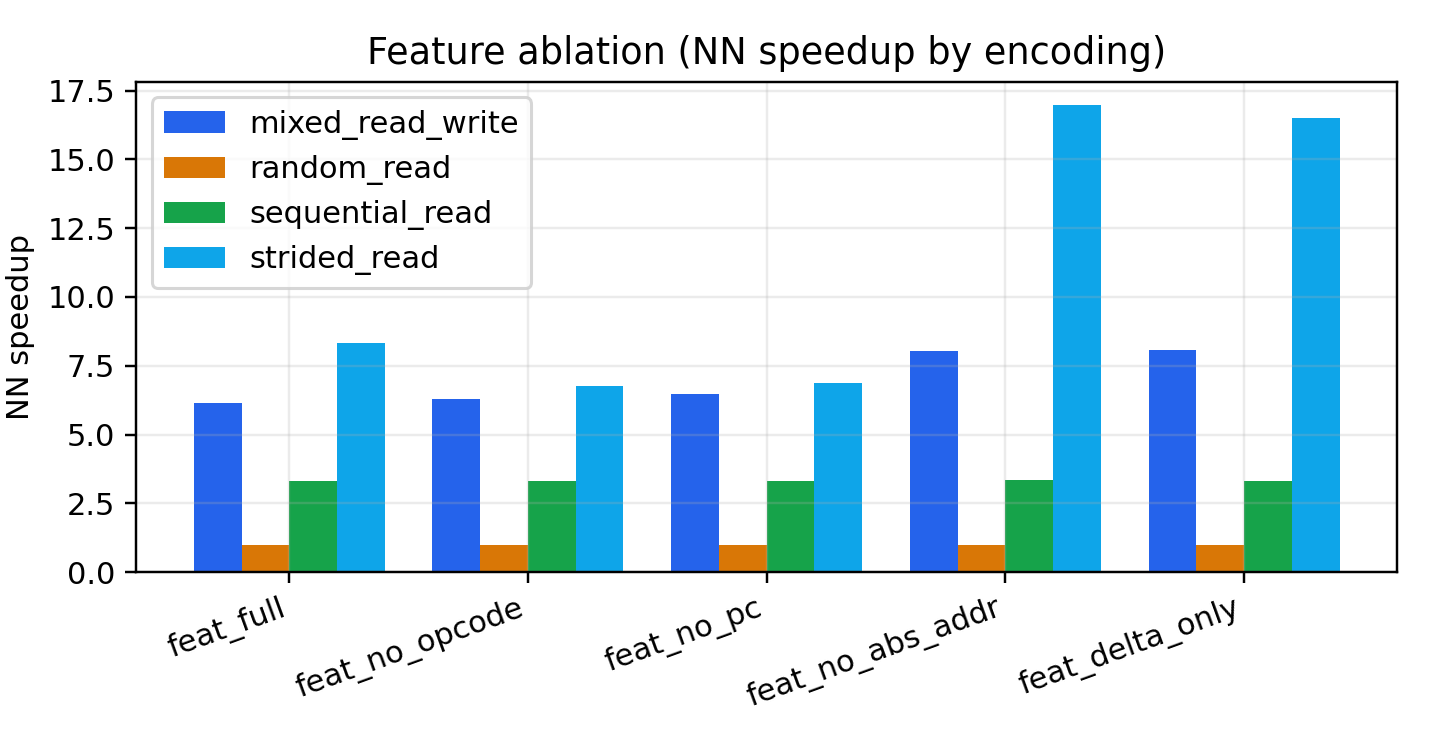
\includegraphics[width=.82\linewidth]{t_feature.png}
\caption{Feature ablation, NN speedup per encoding (grouped by workload).
The absolute-address feature is the only one whose removal increases the
speedup across both workloads.}
\label{fig:feature}
\end{figure}

\begin{table}[t]\centering\small
\caption{Feature ablation, mean of 5 seeds}
\begin{tabular}{lcc}
\toprule
encoding & strided & mixed \\
\midrule
full       & 8.33 & 6.15 \\
no-opcode  & 6.77 & 6.29 \\
no-pc      & 6.87 & 6.47 \\
no-abs-addr& \textbf{16.96} & \textbf{8.04} \\
delta-only & 16.51 & 8.07 \\
\bottomrule
\end{tabular}
\label{tab:feat}
\end{table}

\subsection{Gate design}
Replacing the mean with the \emph{median} recent error and clamping
training deltas to $\pm16$ words is what fixes gather-heavy streams
(Table~\ref{tab:gate}): embedding $1.00{\rightarrow}1.64$x,
kv-cache $1.00{\rightarrow}1.33$x, agent-RAG $1.84{\rightarrow}1.95$x,
with no regression on random (still exactly baseline) or smooth streams.
The adaptive (relative) threshold in (\ref{eq:gate}) additionally keeps
the gate open for large predicted strides (Table~\ref{tab:gate},
Fig.~\ref{fig:gate}).

\begin{figure}[t]\centering
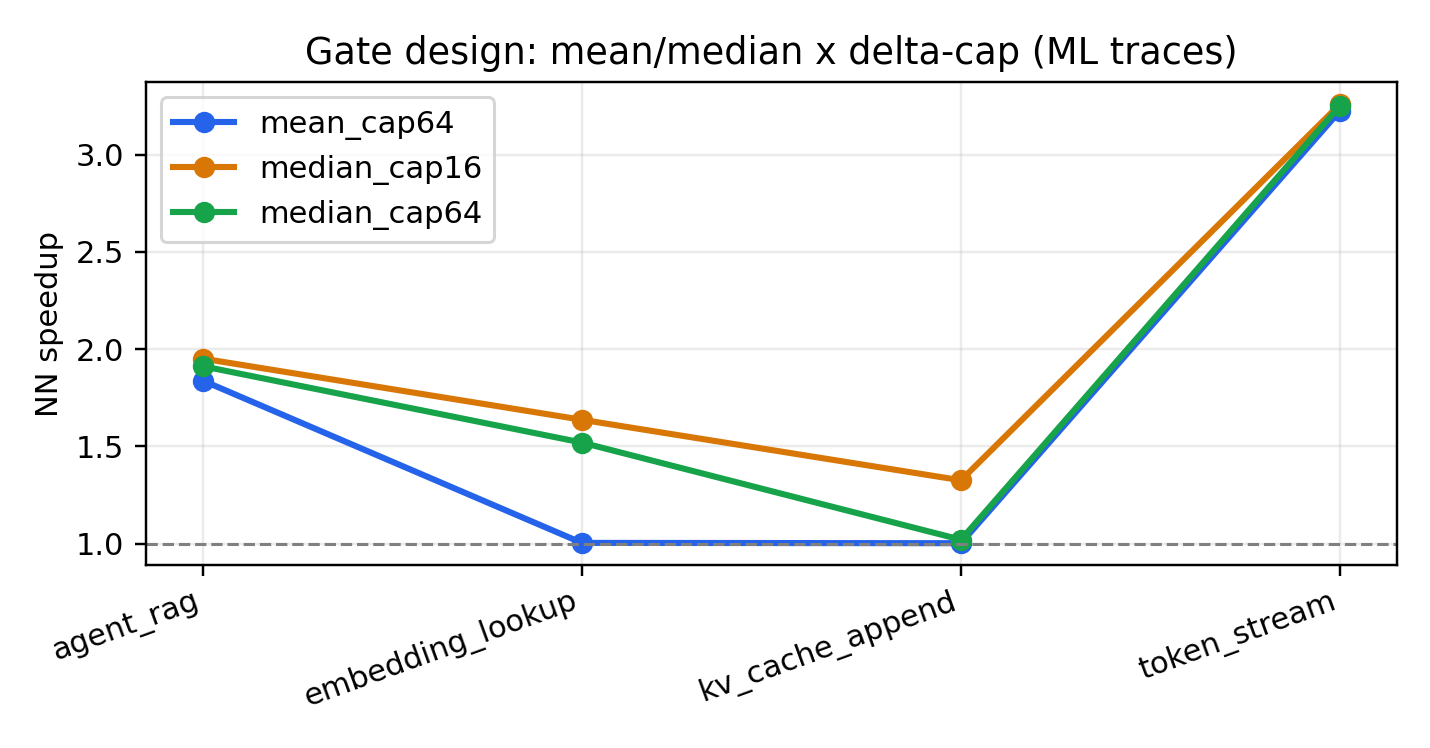
\includegraphics[width=\linewidth]{t_gate.png}
\caption{Gate design on ML/agent traces: NN speedup per workload for the
mean-gate (cap 64) and median-gate (cap 64/16) variants.  The median gate
with $\pm16$-word clamp increases the speedup on embedding and KV-cache
relative to the mean gate.}
\label{fig:gate}
\end{figure}

\begin{table}[t]\centering\small
\caption{Gate robustness on ML/agent traces (mean of 5 seeds)}
\begin{tabular}{lcccc}
\toprule
gate & agent & embed & kv & token \\
\midrule
mean,  cap 64   & 1.84 & 1.00 & 1.00 & 3.23 \\
median,cap 64   & 1.91 & 1.52 & 1.02 & 3.25 \\
median,cap 16   & 1.95 & 1.64 & 1.33 & 3.26 \\
\bottomrule
\end{tabular}
\label{tab:gate}
\end{table}

\subsection{Hyper-parameters, machine sensitivity, backend}
A grid over batch size (8/16/32), hidden width (16/32/64), and learning
rate ($10^{-3}$/1e-2) shows the defaults near-optimal; more warm-up epochs
on the first fit weakly help (8.2$\rightarrow$8.7x on strided).  Sweeping
L1 capacity (16--64 lines), line size (4--16 words), and DRAM latency
(20--80 cycles) preserves every qualitative conclusion, including the
safety property on random (NN $=$ baseline for all settings, while stride
drops below it) (Fig.~\ref{fig:machine}).  For deployment cost, the MLP's
257 parameters fit in a
few cache lines; the pure-NumPy backend is 5--9x faster wall-clock than
an equivalent scikit-learn MLP at statistically identical hit rates
(Fig.~\ref{fig:backend}).

\begin{figure}[t]\centering
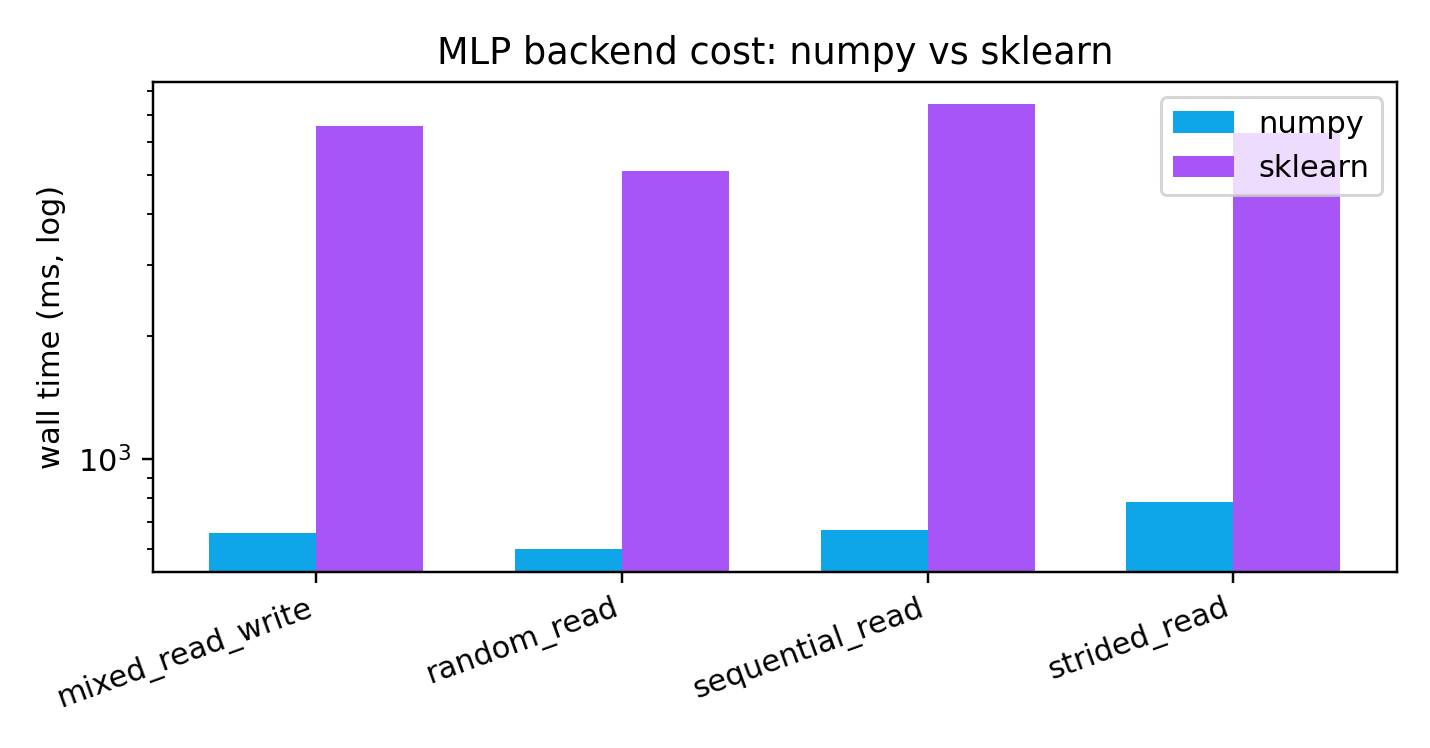
\includegraphics[width=.78\linewidth]{t_backend.png}
\caption{Per-workload wall time for the learned predictor under the NumPy
and scikit-learn backends (log scale).}
\label{fig:backend}
\end{figure}

\begin{figure}[t]\centering
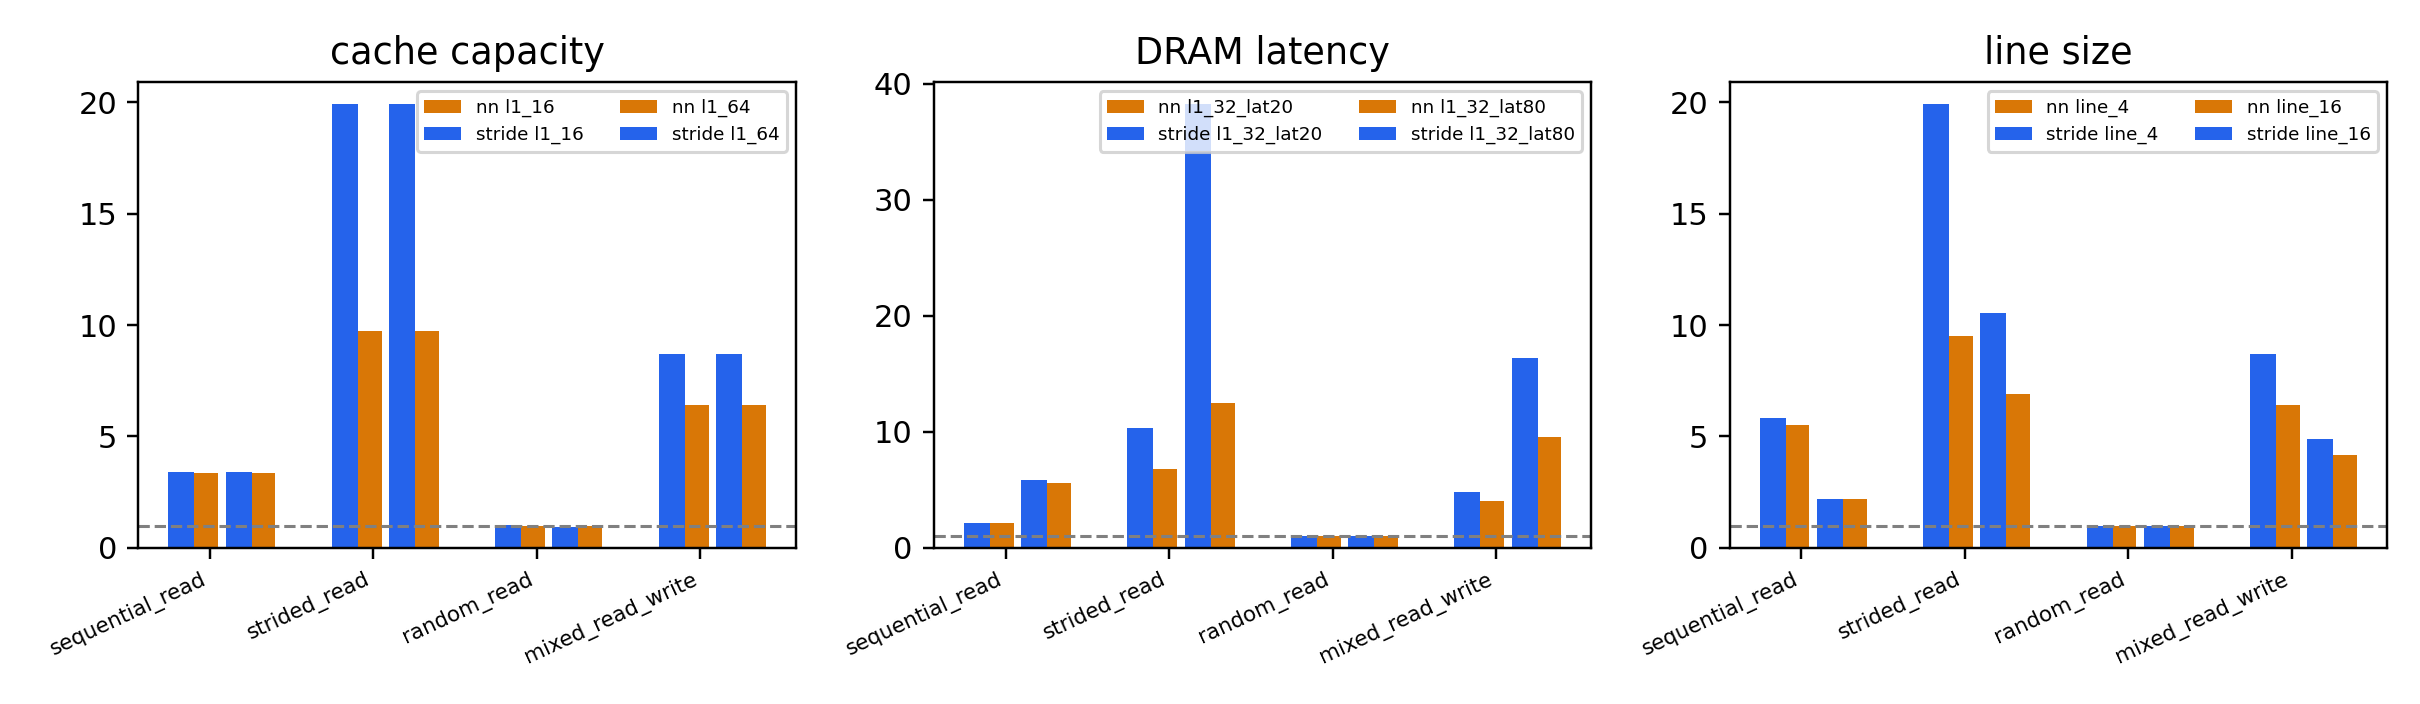
\includegraphics[width=.96\linewidth]{t_machine.png}
\caption{Machine sensitivity: NN vs.\ stride speedup for two settings of
cache capacity, DRAM latency, and line size, on the four dominant
workloads.  The NN's safety on random persists across all settings.}
\label{fig:machine}
\end{figure}

\section{Related work}
\label{sec:rel}
Hardware prefetching is dominated by heuristics: stride/sequence
detection \cite{stride}, signature-path lookahead \cite{SPP}, and
spatial/best-offset units \cite{bingo}.  These excel on their target
streams and are known to be fragile when their assumptions break---the gap
we formalize and measure with the no-prefetch baseline.  Learning-based
predictors were proposed for value and address prediction
\cite{mlpref}; our positioning differs in two ways: we do not try to beat
the heuristics on regular streams (they are near-optimal and we measure
the residual), and we add an explicit \emph{do-not-prefetch} signal,
which is what converts a sometimes-harmful unit into a never-harmful one.

The workloads we target come from the current center of gravity of
memory-bound serving: LLM inference.  Attention and the KV cache dominate
its memory traffic \cite{flash,paged,powerinfer}; the community is already
treating the KV cache as a first-class storage object, with paged and
streamed layouts \cite{paged,cachegen}, quantization that shrinks the
working set \cite{llmint8}, and serving systems that batch and schedule
these sequential generation loops \cite{orca,flexgen}.

Several recent lines are even closer to us and we position against them
explicitly.  On the architecture side, \emph{Pythia} and \emph{Hermes}
\cite{mlmem} learn prefetching \emph{online} with RL/perceptrons and aim to
\emph{outperform} hand-tuned heuristics; we share the online-learning
ingredient but deliberately \emph{do not} compete on speed---classic units
own that---and instead introduce and statistically verify a
\emph{safety} property (never worse than no-prefetching on any seed), which
none of these works declares.  On the LLM-serving side, speculative
decoding \cite{spec} showed that prediction with verification works, and
2025--26 systems use lookahead to \emph{prefetch} exactly the KV blocks or
MoE experts that will be needed next \cite{oasiskv,apex,stmoe}, with at
least one (APEX) using a \emph{learned confidence} to decide whether to
prefetch at all \cite{apex}---conceptually our gate, at a coarser
granularity and aimed at throughput rather than at a no-harm guarantee.
Our microscopic L1-delta formulation and the measurable never-worse
property are, to the best of our knowledge, the pieces none of these
explicitly provide.

\section{Limitations and future work}
\label{sec:lim}
The honest denominator of this work is its simulator: $L=40$-cycle DRAM and
a 32-line L1, not a full ChampSim/SPEC evaluation.  An IPC-level comparison
against published prefetchers on real SPEC/GAP traces requires the port we
list as future work.  Second, the gate is still too conservative on dense
large-stride compute (matmul, mergesort); an adaptive per-region delta
model---learning the active stride and its confidence separately---is the
planned fix.  Third, the MLP's $\approx$26$\,\mu$s prediction is a real,
if small, per-access cost that matters at producer rates; in a hardware
tile it would be trivial, in software less so.  Power/area, a pipelined
front-end, and multi-stream/multi-core behavior remain open.

\section{Reproducibility}
\label{sec:rep}
Every experiment persists \texttt{config.json} and \texttt{manifest.json}
(git revision, library versions, host) next to raw per-seed
\texttt{runs.csv} and aggregated \texttt{summary.csv}; a LaTeX table and
the publication figures are regenerated from the same files.  One command
reruns the full battery (\texttt{python benchmarks/paper\_experiments.py});
a static dashboard (\texttt{dashboard.html}, built by
\texttt{webapp/make\_dashboard.py}) exposes every recorded experiment and
is the fast path for new ablations.

\section{Conclusion}
We asked whether a learned prefetcher adds anything beyond the classics.
The answer our experiments give is a single, statistically robust
property: \emph{a confidence-gated delta predictor is never worse than no
prefetching}, on any stream, with no tuning---whereas every classic
mechanism we modeled degrades below no-prefetch on unpredictable traffic.
When the stream is regular the learned unit recovers most of the
heuristics' win; when it is not, it does no harm.  The safety of
inactivity, we argue, is exactly the property a prefetcher in front of
real, mixed ML/agent workloads needs.

\begin{thebibliography}{12}
\bibitem{memorywall} W.~A. Wulf and S.~A. McKee.
\emph{Hitting the memory wall: implications of the performance of general
purpose computers}. Proceedings of the 22nd Annual International Symposium
on Computer Architecture (ISCA), 1995.
\bibitem{stride} T.-F. Chen and J.-L. Baer.
\emph{Effective hardware-based data prefetching for high-performance
processors}. IEEE Transactions on Computers, 44(5):609--623, 1995.
\bibitem{SPP} J.~Kim, S.~V. Pugsley, P.~V. Gratz, A.~L.~N. Reddy,
C.~Wilkerson, and Z.~Chishti.
\emph{Path confidence based lookahead prefetching}. 49th IEEE/ACM
International Symposium on Microarchitecture (MICRO), 2016.
\bibitem{bingo} M.~Bakhshalipour, P.~Shakerinava, P.~Lotfi-Kamran, and
H.~Sarbazi-Azad.
\emph{Bingo: spatial data prefetching}. 25th IEEE International Symposium
on High Performance Computer Architecture (HPCA), 2019.
\bibitem{mlpref} M.~Hashemi, K.~Swersky, J.~Smith, G.~Ayers, H.~Litz,
J.~Chang, C.~Kozyrakis, and P.~Ranganathan.
\emph{Learning memory access patterns}. 35th International Conference on
Machine Learning (ICML), 2018.
\bibitem{mlmem} R.~Bera, R.~Nadig, and O.~Mutlu.
\emph{Machine learning-driven intelligent memory system design: from
on-chip caches to storage}. IEEE Micro (extended version), 2026;
also arXiv:2603.14583.
\bibitem{oasiskv} C.~Xiao, S.~Cho, J.~We, Z.~Niu, J.~Cheng, Y.~Zhao,
Y.~Kwon, Y.~Xiong, R.~Ma, and J.~Liu.
\emph{OasisKV: scaling in-decode KV cache beyond HBM with lookahead sparse
prefetching}. arXiv:2608.08097, 2026.
\bibitem{apex} A.~Kanani, L.~Badawi, and U.~Y. Ogras.
\emph{APEX: adaptive expert prefetching for memory-efficient edge MoE
inference}. IEEE/ACM CODES+ISSS (ESWEEK), 2026; arXiv:2608.11688.
\bibitem{stmoe} Y.~Zhao, R.~Bunescu, A.~Louri, A.~Karanth, and K.~Wang.
\emph{A spatio-temporal expert prefetching framework for efficient MoE-based
LLM inference}. arXiv:2606.15453, 2026.
\bibitem{paged} W.~Kwon, Z.~Li, S.~Zhuang, Y.~Sheng, L.~Zheng,
C.~H.~Yu, J.~E.~Gonzalez, H.~Zhang, and I.~Stoica.
\emph{Efficient memory management for large language model serving with
PagedAttention}. 29th ACM Symposium on Operating Systems Principles
(SOSP), 2023.
\bibitem{flash} T.~Dao, D.~Y.~Fu, S.~Ermon, A.~Rudra, and C.~R\'e.
\emph{FlashAttention: fast and memory-efficient exact attention with
IO-awareness}. Advances in Neural Information Processing Systems (NeurIPS),
2022.
\bibitem{cachegen} Y.~Liu et al.
\emph{CacheGen: KV cache compression and streaming for fast large language
model serving}. ACM SIGCOMM, 2024.
\bibitem{llmint8} T.~Dettmers, M.~Lewis, Y.~Belkada, and L.~Zettlemoyer.
\emph{LLM.int8(): 8-bit matrix multiplication for transformers at scale}.
Advances in Neural Information Processing Systems (NeurIPS), 2022.
\bibitem{orca} G.-I. Yu, J.~S. Jeong, G.-W. Kim, S.~Kim, and B.-G. Chun.
\emph{Orca: a distributed serving system for transformer-based generative
models}. USENIX OSDI, 2022.
\bibitem{flexgen} Y.~Sheng et al.
\emph{FlexGen: high-throughput generative inference of large language
models with a single GPU}. MLSys, 2023.
\bibitem{spec} Y.~Leviathan, M.~Kalman, and Y.~Matias.
\emph{Fast inference from transformers via speculative decoding}. ICML,
2023.
\bibitem{powerinfer} Y.~Song et al.
\emph{PowerInfer: fast large language model serving with a consumer-grade
GPU}. ICLR, 2024.
\end{thebibliography}

\end{document}